\FloatBarrier

\section{Probabilistic SOM-VAE}

Our proposed model combines ideas from self-organizing maps \citep{Kohonen1998}, variational autoencoders \citep{Kingma2013} and probabilistic models.
In the following, we will lay out the different components of the model and their interactions.


\subsection{Introducing Topological Structure in the Latent Space} \label{sec:SOM-VAE}

\begin{figure}
    \centering
    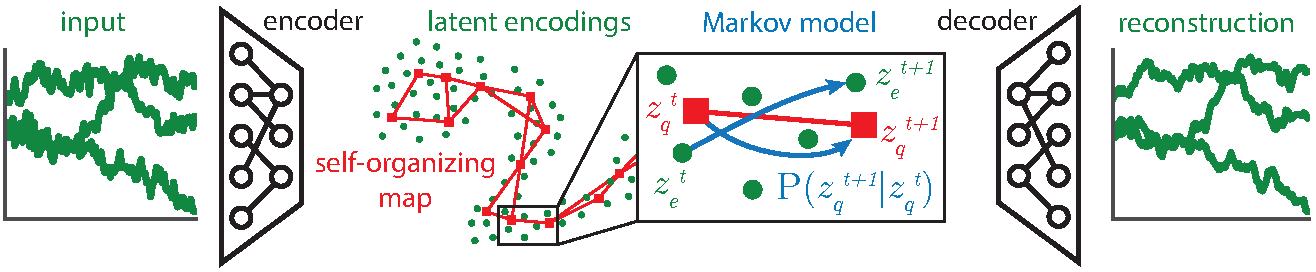
\includegraphics[width=\textwidth]{Overview_SOM-VAE.pdf}
    \caption{Schematic overview of our model architecture. Time series from the data space [green] are encoded by a neural network [black] time-point-wise into the latent space. The latent data manifold is approximated with a self-organizing map (SOM) [red]. In order to achieve a discrete representation, every latent data point ($z_e$) is mapped to its closest node in the SOM ($z_q$). A Markov transition model [blue] is learned to predict the next discrete representation ($z_q^{t+1}$) given the current one ($z_q^t$). The discrete representations can then be decoded by another neural network back into the original data space.}
    \label{fig:overview}
\end{figure}


A schematic overview of our proposed model is depicted in Figure \ref{fig:overview}.
An input $x \in \mathbb{R}^d$ is mapped to a latent encoding $z_e \in \mathbb{R}^m$ (usually $m < d$) by computing $z_e = f_{\theta}(x)$, where $f_{\theta}(\cdot)$ is parameterized by the encoder neural network.
The encoding is then assigned to an embedding $z_q \in \mathbb{R}^m$ in the dictionary of embeddings $E = \lbrace e_1, \dots, e_k \; \vert \; e_i \in \mathbb{R}^m \rbrace$ by sampling $z_q \sim p(z_q | z_e)$.
The form of this distribution is flexible and can be a design choice.
In order for the model to behave similarly to the original SOM algorithm (see below), in our experiments we choose the distribution to be categorical with probability mass 1 on the closest embedding to $z_e$, i.e.\ $p(z_q | z_e) = \mathds{1} \lbrack z_q = \argmin_{e \in E} \| z_e - e\|^2 \rbrack$, where $\mathds{1} \lbrack \cdot \rbrack$ is the indicator function.
A reconstruction $\hat{x}$ of the input can then be computed as $\hat{x} = g_{\phi}(z)$, where $g_{\phi}(\cdot)$ is parameterized by the decoder neural network.
Since the encodings and embeddings live in the same space, one can compute two different reconstructions, namely $\hat{x}_e = g_{\phi}(z_e)$ and $\hat{x}_q = g_{\phi}(z_q)$.

To achieve a topologically interpretable neighborhood structure, the embeddings are connected to form a self-organizing map.
A self-organizing map consists of $k$ nodes $V=\{v_1, \dots , v_k\}$, where every node corresponds to an embedding in the data space $e_v \in \mathbb{R}^d$ and a representation in a lower-dimensional discrete space $m_v \in M$, where usually $M \subset \mathbb{N}^2$.
During training on a data set $\mathcal{D} = \{x_1, \dots ,x_n\}$, a winner node $\tilde{v}$ is chosen for every point $x_i$ according to $\tilde{v} = \argmin_{v \in V} \| e_v - x_i \|^2$.
The embedding vector for every node $u \in V$ is then updated according to $e_u \leftarrow e_u + N(m_u,m_{\tilde{v}}) \eta (x_i - e_u)$, where $\eta$ is the learning rate and $N(m_u, m_{\tilde{v}})$ is a neighborhood function between the nodes defined on the representation space $M$.
There can be different design choices for $N(m_u, m_{\tilde{v}})$.
A more thorough review of the self-organizing map algorithm is deferred to the appendix (Sec.~\ref{sec:SOMs}).

We choose to use a two-dimensional SOM because it facilitates visualization similar to \citet{Tirunagari2015}.
Since we want the architecture to be trainable end-to-end, we cannot use the standard SOM training algorithm described above.
Instead, we devise a loss function term whose gradient corresponds to a weighted version of the original SOM update rule (see below).
We implement it in such a way that any time an embedding $e_{i,j}$ at position $(i,j)$ in the map gets updated, it also updates all the embeddings in its immediate neighborhood $N(e_{i,j})$.
The neighborhood is defined as $N(e_{i,j}) = \{ e_{i-1,j}, e_{i+1,j}, e_{i,j-1}, e_{i,j+1} \}$ for a two-dimensional map.

The loss function for a single input $x$ looks like
%
\begin{equation} \label{eq:L_somvae}
	\mathcal{L}_{\text{SOM-VAE}}(x, \hat{x}_q, \hat{x}_e) = \mathcal{L}_{\text{reconstruction}}(x, \hat{x}_q, \hat{x}_e) + \alpha \, \mathcal{L}_{\text{commitment}}(x) + \beta \, \mathcal{L}_{\text{SOM}}(x)
\end{equation}
%
where $x$, $z_e$, $z_q$, $\hat{x}_e$ and $\hat{x}_q$ are defined as above and $\alpha$ and $\beta$ are weighting hyperparameters.

Every term in this function is specifically designed to optimize a different model component.
The first term is the reconstruction loss $\mathcal{L}_{\text{reconstruction}}(x, \hat{x}_q, \hat{x}_e) = \| x - \hat{x}_q \|^2 + \| x - \hat{x}_e \|^2$.
The first subterm of this is the discrete reconstruction loss, which encourages the assigned SOM node $z_q(x)$ to be an informative representation of the input.
The second subterm encourages the encoding $z_e(x)$ to also be an informative representation.
This ensures that all parts of the model have a fully differentiable credit assignment path to the loss function, which facilitates training.
Note that the reconstruction loss corresponds to the evidence lower bound (ELBO) of the VAE part of our model \citep{Kingma2013}.
Since we assume a uniform prior over $z_q$, the KL-term in the ELBO is constant w.r.t.\ the parameters and can be ignored during optimization.

The term $\mathcal{L}_{\text{commitment}}$ encourages the encodings and assigned SOM nodes to be close to each other and is defined as $\mathcal{L}_{\text{commitment}}(x) = \| z_e(x) - z_q(x) \|^2$.
Closeness of encodings and embeddings should be expected to already follow from the $\mathcal{L}_{\text{reconstruction}}$ term in a fully differentiable architecture.
However, due to the non-differentiability of the embedding assignment in our model, the $\mathcal{L}_{\text{commitment}}$ term has to be explicitly added to the objective in order for the encoder to get gradient information about $z_q$.

The SOM loss $\mathcal{L}_{\text{SOM}}$ is defined as $\mathcal{L}_{\text{SOM}}(x) = \sum_{\tilde{e} \in N(z_q(x))} \| \tilde{e} - \text{sg}[z_e(x)] \|^2$, where $N(\cdot)$ is the set of neighbors in the discrete space as defined above and $\text{sg}[\cdot]$ is the gradient stopping operator that does not change the outputs during the forward pass, but sets the gradients to 0 during the backward pass.
It encourages the neighbors of the assigned SOM node $z_q$ to also be close to $z_e$, thus enabling the embeddings to exhibit a self-organizing map property, while stopping the gradients on $z_e$ such that the encoding is not pulled in the direction of the neighbors.
This term enforces a neighborhood relation between the discrete codes and encourages all SOM nodes to ultimately receive gradient information from the data.
The gradient stopping in this term is motivated by the observation that the data points themselves do not get moved in the direction of their assigned SOM node's neighbors in the original SOM algorithm either (see above).
We want to optimize the embeddings based on their neighbors, but not the respective encodings, since any single encoding should be as close as possible to its assigned embedding and not receive gradient information from any other embeddings that it is not assigned to.
Note that the gradient update of a specific SOM node in this formulation depends on its distance to the encoding, while the step size in the original SOM algorithm is constant.
It will be seen that this offers some benefits in terms of optimization and convergence (see Sec. \ref{sec:clustering_benchmark}).


\subsection{Overcoming the Non-Differentiability}\label{sec:non-differentiability}

The main challenge in optimizing our architecture is the non-differentiability of the discrete cluster assignment step.
Due to this, the gradients from the reconstruction loss cannot flow back into the encoder.
A model with a similar problem is the recently proposed vector-quantized VAE (VQ-VAE) \citep{Oord2017}.
It can be seen as being similar to a special case of our SOM-VAE model, where one sets $\beta = 0$, i.e. disables the SOM structure.

In order to mitigate the non-differentiability, the authors of the VQ-VAE propose to copy the gradients from $z_q$ to $z_e$.
They acknowledge that this is an \emph{ad hoc} approximation, but observed that it works well in their experiments.
Due to our smaller number of embeddings compared to the VQ-VAE setup, the average distance between an encoding and its closest embedding is much larger in our case.
The gradient copying (see above) thus ceases to be a feasible approximation, because the true gradients at points in the latent space which are farther apart will likely be very different.

In order to still overcome the non-differentiability issue, we propose to add the second reconstruction subterm to $\mathcal{L}_{\text{reconstruction}}$, where the reconstruction $\hat{x}_e$ is decoded directly from the encoding $z_e$.
This adds a fully differentiable credit assignment path from the loss to the encoder and encourages $z_e$ to also be an informative representation of the input, which is a desirable model feature.
Most importantly, it works well in practice (see Sec.\ \ref{sec:clustering_benchmark}).

Note that since $z_e$ is continuous and therefore much less constrained than $z_q$, this term is optimized easily and becomes small early in training.
After that, mostly the $z_q$-term contributes to $\mathcal{L}_{\text{reconstruction}}$.
One could therefore view the $z_e$-term as an initial encouragement to place the data encodings at sensible positions in the latent space, after which the actual clustering task dominates the training objective.



\subsection{Encouraging Smoothness over Time}\label{sec:probabilistic_model}

Our ultimate goal is to predict the development of time series in an interpretable way.
This means that not only the state representations should be interpretable, but so should be the prediction as well.
To this end, we use a temporal probabilistic model.

Learning a probabilistic model in a high-dimensional continuous space can be challenging.
Thus, we exploit the low-dimensional discrete space induced by our SOM to learn a temporal model.
For that, we define a system state as the assigned node in the SOM and then learn a Markov model for the transitions between those states.
The model is learned jointly with the SOM-VAE, where the loss function becomes
%
\begin{equation}\label{eq:L_prob}
    \mathcal{L}(x^{t-1}, x^t, \hat{x}_q^t, \hat{x}_e^t) = \mathcal{L}_{\text{SOM-VAE}}(x^t, \hat{x}_q^t, \hat{x}_e^t) + \gamma \, \mathcal{L}_{\text{transitions}}(x^{t-1}, x^t) + \tau \, \mathcal{L}_{\text{smoothness}}(x^{t-1}, x^t)
\end{equation}
%
with weighting hyperparameters $\gamma$ and $\tau$.

The term $\mathcal{L}_{\text{transitions}}$ encourages the probabilities of actually observed transitions to be high.
It is defined as $\mathcal{L}_{\text{transitions}}(x^{t-1}, x^t) = - \log P_{M} (z_q(x^{t-1}) \rightarrow z_q(x^t))$, with $P_{M} (z_q(x^{t-1}) \rightarrow z_q(x^t))$ being the probability of a transition from state $z_q(x^{t-1})$ to state $z_q(x^t)$ in the Markov model.

The term $\mathcal{L}_{\text{smoothness}}$ encourages the probabilities for transitions to nodes that are far away from the current data point to be low or respectively the nodes with high transition probabilities to be proximal.
It achieves this by taking large values only for transitions to far away nodes that have a high probability under the model.
It is defined as $\mathcal{L}_{\text{smoothness}}(x^{t-1}, x^t) = \mathbb{E}_{P_{M} \left( z_q(x^{t-1}) \rightarrow \tilde{e} \right) } \left[ \| \tilde{e} - z_e(x^t) \|^2 \right]$.
The probabilistic model can inform the evolution of the SOM through this term which encodes our prior belief that transitions in natural data happen smoothly and that future time points will therefore mostly be found in the neighborhood of previous ones.
In a setting where the data measurements are noisy, this improves the clustering by acting as a temporal smoother.

